\documentclass{article}\usepackage[]{graphicx}\usepackage[]{color}
%% maxwidth is the original width if it is less than linewidth
%% otherwise use linewidth (to make sure the graphics do not exceed the margin)
\makeatletter
\def\maxwidth{ %
  \ifdim\Gin@nat@width>\linewidth
    \linewidth
  \else
    \Gin@nat@width
  \fi
}
\makeatother

\definecolor{fgcolor}{rgb}{0.345, 0.345, 0.345}
\newcommand{\hlnum}[1]{\textcolor[rgb]{0.686,0.059,0.569}{#1}}%
\newcommand{\hlstr}[1]{\textcolor[rgb]{0.192,0.494,0.8}{#1}}%
\newcommand{\hlcom}[1]{\textcolor[rgb]{0.678,0.584,0.686}{\textit{#1}}}%
\newcommand{\hlopt}[1]{\textcolor[rgb]{0,0,0}{#1}}%
\newcommand{\hlstd}[1]{\textcolor[rgb]{0.345,0.345,0.345}{#1}}%
\newcommand{\hlkwa}[1]{\textcolor[rgb]{0.161,0.373,0.58}{\textbf{#1}}}%
\newcommand{\hlkwb}[1]{\textcolor[rgb]{0.69,0.353,0.396}{#1}}%
\newcommand{\hlkwc}[1]{\textcolor[rgb]{0.333,0.667,0.333}{#1}}%
\newcommand{\hlkwd}[1]{\textcolor[rgb]{0.737,0.353,0.396}{\textbf{#1}}}%

\usepackage{framed}
\makeatletter
\newenvironment{kframe}{%
 \def\at@end@of@kframe{}%
 \ifinner\ifhmode%
  \def\at@end@of@kframe{\end{minipage}}%
  \begin{minipage}{\columnwidth}%
 \fi\fi%
 \def\FrameCommand##1{\hskip\@totalleftmargin \hskip-\fboxsep
 \colorbox{shadecolor}{##1}\hskip-\fboxsep
     % There is no \\@totalrightmargin, so:
     \hskip-\linewidth \hskip-\@totalleftmargin \hskip\columnwidth}%
 \MakeFramed {\advance\hsize-\width
   \@totalleftmargin\z@ \linewidth\hsize
   \@setminipage}}%
 {\par\unskip\endMakeFramed%
 \at@end@of@kframe}
\makeatother

\definecolor{shadecolor}{rgb}{.97, .97, .97}
\definecolor{messagecolor}{rgb}{0, 0, 0}
\definecolor{warningcolor}{rgb}{1, 0, 1}
\definecolor{errorcolor}{rgb}{1, 0, 0}
\newenvironment{knitrout}{}{} % an empty environment to be redefined in TeX

\usepackage{alltt} % JASA requires 12 pt font for manuscripts
%\usepackage{JASA_manu}        % For JASA manuscript formatting

%\usepackage{endfloat} % just for while I am writing

% for citations
\usepackage[authoryear]{natbib} % natbib required for JASA
\usepackage[colorlinks=true, citecolor=blue, linkcolor=blue]{hyperref}

% for the fancy tables with the icons
%\usepackage[margin=1.0in]{geometry}% http://ctan.org/pkg/margin
\usepackage{booktabs}% http://ctan.org/pkg/booktabs
\usepackage{array}% http://ctan.org/pkg/array
\newcolumntype{M}{>{\centering\arraybackslash}m{\dimexpr.05\linewidth-2\tabcolsep}}



%\definecolor{Blue}{rgb}{0,0,0.5}
\newcommand{\hh}[1]{{\color{magenta} #1}}
\newcommand{\al}[1]{{\color{red} #1}}

% fonts
%\usepackage{kpfonts}

% for figures
\usepackage{graphicx}
\DeclareGraphicsExtensions{.eps, .pdf}
\graphicspath{{figures/}}

\usepackage{wrapfig,float}
\usepackage{caption}
\usepackage{subcaption}

% help with editing and coauthoring
\usepackage{todonotes}
\newcommand{\alnote}[1]{\todo[inline,color=green!40]{#1}}
\newcommand{\hhnote}[1]{\todo[inline,color=magenta!40]{#1}}

% title formatting
\usepackage[compact,small]{titlesec}

% page formatting
\usepackage[margin = 1in]{geometry}
\usepackage[parfill]{parskip}

% line spacing
\usepackage{setspace}
\doublespace

% For math typsetting
\usepackage{bm}
\usepackage{amstext}
\usepackage{amssymb}
\usepackage{amsmath}
\usepackage{amsfonts}
\usepackage{multirow}

% A few commands to make typing less tedious
\newcommand{\inv}{\ensuremath{^{-1}}}
\newcommand{\ginv}{\ensuremath{^{-}}}
\newcommand{\trans}{\ensuremath{^\prime}}
\newcommand{\E}{\ensuremath{\mathrm{E}}}
\newcommand{\var}{\ensuremath{\mathrm{Var}}}
\newcommand{\cov}{\ensuremath{\mathrm{Cov}}}


\title{Variations of Q-Q Plots -- the eyes have it!}

\author{Adam Loy, Lendie Follett, Heike Hofmann}
\IfFileExists{upquote.sty}{\usepackage{upquote}}{}
\begin{document}
\maketitle
\begin{abstract}
this paper holds two messages: 
a) our eyes are well suited to assess distributional assumptions. We  objectively measure  power and sensitivity of Q-Q plots using lineup tests. 
At the example of normal distributions we can show that Q-Q plots are better at identifying non-normality than some prominent tests of normality, such as Shapiro-Wilks,  Anderson-Darling,  Kolmogorov-Smirnov, Lilliefors, or  Cramer-von-Mises.

b) Out of the variations discussed, rotated Q-Q plots perform significantly worse than the other two variants. This is surprising, because cognitive theory tells us, that rotated plots should be better suited in assessing the difference between empirical and hypothesized  distribution.
\end{abstract}











%------------------------------------------------------------------------------------
\section{Introduction}
%------------------------------------------------------------------------------------

Standard quantile-quantile (Q-Q) plots \citep{Wilk:1968} are an essential tool for  visually evaluating a specific distributional assumption. In a Q-Q plot we plot the empirical distribution against the expected quantiles from the assumed distribution. The line of identity therefore represents the theoretical distribution and points show quantiles of the empirical distributions. Deviations from the theoretical distribution then manifest themselves as vertical differences between points and the line of identity. This difference is featured in a series of distributional tests. More formally, let $F_n$ be the empirical distribution function (ECDF) based on a sample size of $n$, and $F$ be the hypothesized/true distribution. The absolute difference between the two distribution functions for each sample point, $\left| F_n(x_i) - F(x_i) \right|$, is then the main contributor for the test statistics of the Kolmogorov-Smirnov \cite[KS-test,][]{kolmogorov:1933, smirnov:1948}, the Lilliefors \cite[LF-test, ][]{lilliefors}, the Anderson-Darling \citep[AD-test,][]{adtest:1954}, and the Cram\'{e}r-von-Mises test \citep[CVM-test,][]{cramer:1928, mises:1928}, as shown in table~\ref{tab:tests}.

The KS test uses the maximal  difference, which is displayed as the maximal vertical extent between the line of identity and the data points in a Q-Q plot, regardless of the range of the sample, i.e. a difference $D$ observed at either tail of the distribution carries the same weight and is interpreted in the same way as a difference $D$ in the center of the distribution. While the KS test allows for adjusting parameters of the normal distribution to sample mean and variance, it is more appropriate to use LF for this purpose. LF and KS share the same test statistic, but the null distributions vary.  AD and CVM  are both based on the total area between the line of identity and the empirical distribution function. Compared to the KS  test,  the CVM test downplays the effects in the tails of a (normal) distribution, while Anderson-Darling upregulates the tail effect again due to its additional weighting of $1/\left(F(x)(1 - F(x)\right)$ across the range of the sample. 
The Shapiro-Wilks test does not fit this scheme, but has been shown to be the most powerful in assessing non-normality \citep{stephens:1974, razali:2011}.
\begin{table}
\centering
\begin{tabular}{lrl}\hline
Test && Statistic\\\hline\hline
Kolmogorov-Smirnov & $D =$ & $ \sup_{1 \le i \le n} \left | F_n(x_i) - F(x_i)\right|$ \\
Lilliefors & $D =$ & $ \sup_{1 \le i \le n} \left | F_n(x_i) - F(x_i)\right|$ \\
Anderson-Darling & $A =$ & $ n \int_{-\infty}^{+\infty} \left | F_n(x) - F(x)\right|^2/\left(F(x)(1 - F(x)\right) dF(x)$\\
Cram\'{e}r-von-Mises & $C =$ & $n \int_{-\infty}^{+\infty} \left | F_n(x) - F(x)\right|^2 dF(x)$ \\\hline
\end{tabular}
\caption{\label{tab:tests} Four prominent tests for normality based on the difference between empirical and hypothesized distribution function. An overview of the performance and power of these tests can be found in \citet{stephens:1974}.}
\end{table}
%
We will be making use of these tests to assess the effectiveness of different variations of standard Q-Q plots.


\hhnote{How are Q-Q plots constructed? - We need to introduce this with a bit more formality.}

\hhnote{How are Q-Q plots interpreted?} \hh{A sample $x$ is considered as being consistent with a normal distribution, if empirical and empirical quantiles fall close to  a straight line. For all of the variations of Q-Q plots considered in this paper, a line representing the theoretical distribution is drawn explicitly. Closeness can  be assessed visually based on whether the points fall inside the envelope of 95\%  pointwise confidence intervals. Slope and intercept of the line show standard deviations and mean of the hypothesized/theoretical distribution.  }

\hh{XXX paragraphs above and below out of order}

Examples of the three versions are displayed in Figure~\ref{qqplots} and include (from left to right): a \emph{control} Q-Q plot, a \emph{standard} Q-Q plot with an added grey band representing a 95\% pointwise confidence region \hh{cite Meeker} based on the estimated standard error of the order statistics for an independent sample from the theoretical distribution, and a \emph{rotated} (i.e., detrended) Q-Q plot. All Q-Q plots in Figure~\ref{qqplots} are constructed from the same data. 

\begin{figure}
\centering
% <<qqplots, dependson='functions', fig.width=2.75, fig.height=2.75, out.width='0.3\\textwidth', echo=FALSE, include=TRUE>>=
% dframe <- read.csv("lineup-data/data-1-1-1-20-2-14-5.csv")
% library(ggplot2)
% dframe$.sample <- "Control"
% ctrl_lineup(subset(dframe, .sample_outer==5))
% dframe$.sample <- "Standard"
% std_lineup(subset(dframe, .sample_outer==5))
% dframe$.sample <- "Rotated"
% rot_lineup(subset(dframe, .sample_outer==5))
% @
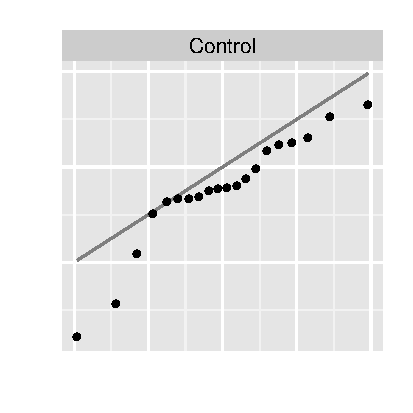
\includegraphics[width=0.3\textwidth]{qqplots1}
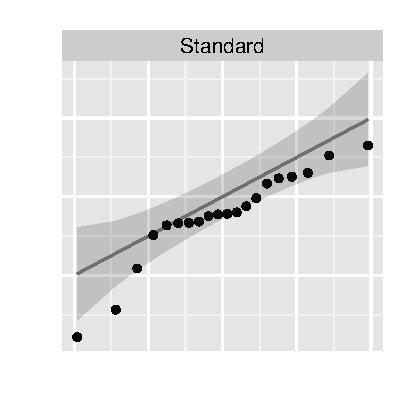
\includegraphics[width=0.3\textwidth]{qqplots2}
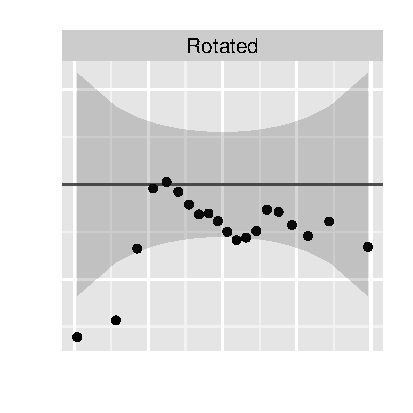
\includegraphics[width=0.3\textwidth]{qqplots3}
\caption{ \label{qqplots} Three versions of Q-Q plots: control, standard, and rotated.}
\end{figure}
\alnote{Setting up the Q-Q plot, visual perception motivation of the study, and visual inference.}

\hhnote{Cognitive perception:}
\hh{In de-trended Q-Q plots $x$-values are given by the quantiles of the empirical distribution as in regular Q-Q plots. $y$-values are given by the difference between empirical and theoretical distributiom. The line of the theoretical distribution therefore coincides with the $x$ axis. 

In assessing differences between points and lines, onlookers have a tendency to evaluate shortest, i.e.~orthogonal, distances, even if asked to evaluate differences based on vertical distances \citep{sineillusion, robbins:2005, cleveland:1984}. 
In de-trended Q-Q plots vertical difference between empirical and theoretical distribution coincides with orthogonal distance. 
De-trending should therefore aid the visual assessment between empirical CDF and theoretical CDF. It is also in line with the standard graphical recommendation to directly plot the aspect of the data we want to show rather than asking audiences to derive it \citep{wainer:2000}.
}

\hh{In order to objectively evaluate  the three designs and quantify their effectiveness we make use of {\it lineup tests}.}

Lineup tests have been introduced by \citet{buja:2009hp} to evaluate and quantify the significance of graphical findings. The idea behind a lineup test is that of a police lineup: the chart of the observed data is placed randomly among a set of so called null charts, which show data created consistently with the null hypothesis. \hhnote{null hypothesis here is either that F is standard normal or F is normal with parameters based on sample mean and variance.}
If the `suspect' -- i.e. the plot of the observed data -- can be identified from the null charts, this is evidence against the null hypothesis. Multiple identifications of the data by independent observers then lead to a rejection of the null hypothesis.
The lineup protocol also allows for an assessment of the power of a lineup \citep{mahbub:2013}. 
%as the probability that in $N$ independent evaluations observers 
In $N$ independent evaluations, the probability that observers
choose the true plot more than $x_\alpha$ times is
\begin{equation}\label{eqn:power}
\widehat{\text{Power}} = \text{Power}_{N} = 1 - F_{X} (x_{\alpha}),
\end{equation}
where $F_X$ is the distribution of $X$ and $x_\alpha$ is the critical value for a given significance level of $\alpha$, i.e. $P(X >  x_{\alpha}) \le \alpha$. $X$ is composed of the sum of $N$ observers' (binary) decisions $X_i \sim B_{1, p_i}$, where  $p_i$ is the probability that individual $i$ chooses the data plot. This probability  depends both on the strength of the signal in the data plot and an individual's visual ability.
Assessing this ability requires that each individual evaluates multiple lineups. 
If that is not possible, we have to assume that all participants share the same ability, and the power calculation in Equation~\ref{eqn:power} simplifies to $1 - B_{N, \hat{p}}(x_\alpha)$, where $\widehat{p}$ is an estimate for the probability of choosing the data plot for a specific lineup. Similar to classical inference, we can make use of power to assess sensitivity of tests. This allows us to make decisions about designs for particular tasks by evaluating lineups displaying  the same data in different types of displays \citep{Hofmann:2012ts}. 

%------------------------------------------------------------------------------------
\section{Investigating Q-Q plots visually}\label{sec:qqplot}
%------------------------------------------------------------------------------------

%------------------------------------------------------------------------------------
\subsection{Method}
%------------------------------------------------------------------------------------

To further \al{develop} the assessment of normality using lineups, we conducted a study comparing the three different versions of the Q-Q plot.
%We are testing three different versions of a Q-Q plot, 


To investigate the power of the three different Q-Q plot versions, we sample data from a $t$ distribution with varying degrees of freedom and sample sizes, and include a Q-Q plot of this data in a lineup of null charts drawn from standard normal samples of the same size.
For lineup tests it is of extreme importance to consider the generation of the null sets and the construction of the plots in the lineup. 

\begin{tabular}{lp{5.25in}}
$F = N(0,1)$ & reference line and envelope are identical across all panels, i.e.~panels all have the same scale. \\
$F = N(\bar{X},S^2)$ & reference line and envelope are drawn based on sample mean and variance of the data sample; all panels have the same scale. Note that we employ robust estimators in estimating $\bar{X}$ and $S^2$.  $S$ is based on the interquartile range of the sample, as is common in the construction of Q-Q plots.
\end{tabular}

\begin{figure}[hbt]


\begin{subfigure}{0.5\textwidth}
\begin{knitrout}
\definecolor{shadecolor}{rgb}{0.969, 0.969, 0.969}\color{fgcolor}
\includegraphics[width=\maxwidth]{figure/unnamed-chunk-1} 

\end{knitrout}

\end{subfigure}
\begin{subfigure}{0.5\textwidth}
\begin{knitrout}
\definecolor{shadecolor}{rgb}{0.969, 0.969, 0.969}\color{fgcolor}
\includegraphics[width=\maxwidth]{figure/unnamed-chunk-2} 

\end{knitrout}

\end{subfigure}
\caption{\label{fig:lps} Lineup plots of standard Q-Q plots. The underlying data is identical, but on the left reference lines and envelopes are based on a standard normal distribution. Reference lines and envelopes for the lineup on the right are based on a normal distribution $N(\bar{X}, S^2)$, the estimates of the data.
The observed data in both lineups is displayed in panel \#$(3^2 - 3)$. }
\end{figure}


To explore the results of this study we must first define some additional notation.

\alnote{We can give a description of the MTurk study here.}

%------------------------------------------------------------------------------------
\subsection{Results}
%------------------------------------------------------------------------------------


Let $X_i \sim B_{1, \pi_i}, 1 \le i \le n$, where $X_i$ is the binary decision on the $i$th evaluation and $\pi_i$ is the probability with which the observer chooses the data plot. This probability is influenced by a number of factors:

\begin{center}
\begin{tabular}{lp{5in}}
$\tau$ & the design used in the lineup (Control, Standard, Rotated), \\
&  the specific parameters under which the data for the lineup were created: \\
&  $\delta$ \ \ \ degrees of freedom (2, 5, 10) {of the $t$ distribution} and \\
&  $\nu$  \ \ \ sample size (20, 30, 50, 75), \\
$d$ &  the level of difficulty based on the actual sample, and \\
$u$ & the users' subjective abilities.
 \end{tabular}
\end{center}
%

%
The combination of different levels of sample size and degrees of freedom of the $t$ distribution result in 12 parameter settings. Under each setting, we sampled data twice; additionally, we sampled two sets of null data for each sample, yielding 48 different sets of data, which we render in each of the variations, yielding 144 different lineups. 
Using  Amazon MTurk \citep{amazon}, 674 participants were each asked to evaluate ten different lineups each. 
\hh{weights? We dealt with multiple answers to lineups that offered this choice by using a weighting variabe with reciprocal values of the number of answers given by a participant.}








\begin{figure}
\centering
\begin{subfigure}[b]{.3\textwidth}
\begin{knitrout}
\definecolor{shadecolor}{rgb}{0.969, 0.969, 0.969}\color{fgcolor}
\includegraphics[width=\maxwidth]{figure/unnamed-chunk-3} 

\end{knitrout}

\end{subfigure}
\begin{subfigure}[b]{.3\textwidth}
\begin{knitrout}
\definecolor{shadecolor}{rgb}{0.969, 0.969, 0.969}\color{fgcolor}
\includegraphics[width=\maxwidth]{figure/unnamed-chunk-4} 

\end{knitrout}

\end{subfigure}
\begin{subfigure}[b]{.3\textwidth}
\begin{knitrout}
\definecolor{shadecolor}{rgb}{0.969, 0.969, 0.969}\color{fgcolor}
\includegraphics[width=\maxwidth]{figure/unnamed-chunk-5} 

\end{knitrout}

\end{subfigure}
\caption{\label{fig:compare}Proportions of successful evaluation of the same data in the three different variations of Q-Q plots. Standard and control displays exhibit the highest correlation. Rotated Q-Q plots agree with decisions made based on Q-Q plots in the control or standard design, but display lower rates of correct responses in the `middle' field. Significances are based on lineup evaluations in the standard design. }
\end{figure}

\begin{figure}
\centering
%\begin{subfigure}[t]{.3\textwidth}
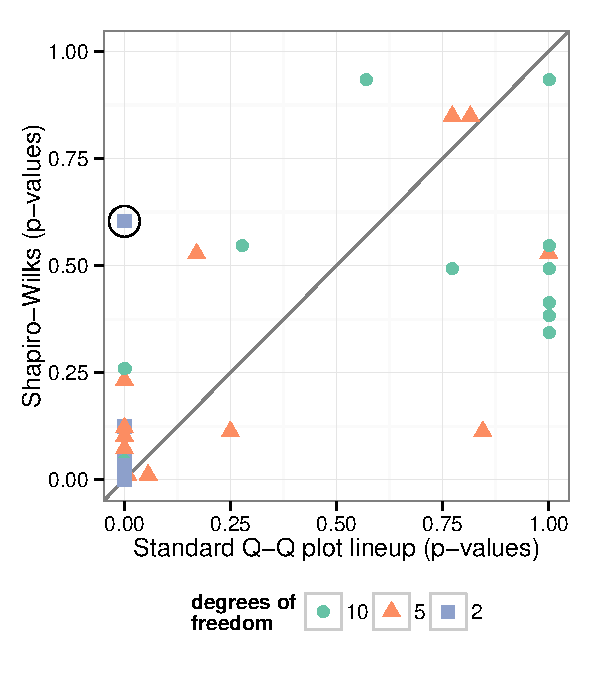
\includegraphics[width=.5\textwidth]{figures/fig:visnorm.pdf} 
%\vfill
%\end{subfigure}
%\begin{subfigure}[t]{.6\textwidth}
%\includegraphics[width=\textwidth]{figures/filebab632311351-multiple-svg.pdf}
%\end{subfigure}
\caption{\label{fig:visnorm} Scatterplot of $p$-values from Shapiro-Wilks and estimated $p$-values from lineups of Standard Q-Q plots. The circled observation on the left corresponds to a sample that shows highly significant deviations from normality under the lineup test, but is not significant under Shapiro Wilks (nor any of the normality tests except for KS). The lineup for the testing is shown on the left hand side of figure~\ref{fig:lps}.
\hhnote{We probably need to exchange this plot by the visual $p$-values based on the lineups adjusted by the standard deviation.}
%\hh{XXX This is potentially problematic - the lineup flares up so strongly, because the lineup is testing against standard normal, while the normal tests are testing for the family - the KS test discussed here is the Lilliefors extension. The actual KS test is significant for this dataset, but then only rejects 3 others. Looking at the two side by side lineups the problem is smaller than it initially seemed. Should we re-run a subset of the data with the scale free lineups?}
}
\end{figure}
Figure~\ref{fig:compare} shows proportions of correct evaluations of the lineups under the three different variations of Q-Q plots. All three versions provide highly correlated results, and largely coincide for extreme decisions (all correct/all wrong evaluations). In the middle range rotated Q-Q plots perform significantly worse than either standard or control Q-Q plots. Lineups including data samples from a $t_2$-distribution  are all rejected in lineups under the standard design, while most of the $t_{10}$ samples go undetected. 

\hh{XXX lead into the model}

We model the probability of selecting the data plot from the lineup, $\pi$, with the help of model $M_1$:
\[
g(\pi_i) = \mu + \tau_{j(i)} +\delta_{k(i)}+ \nu_{s(i)} + u_{u(i)} + d_{d(i)}
\]
where $g$ is the logit link function, and $j(.), k(.), s(.), u(.)$, and $d(.)$ are all indexing functions that relate evaluation $i$ to the corresponding levels in the factor variables, to the observer, or a particular data sample. More specifically, $j(i) \in \{$Control, Standard, Rotated$\}$; $k(i) \in \{2,5,10\}$; $s(i) \in \{20, 30, 50, 75\}$; $u(i)$ maps to the participant's id of the $i$th evaluation and $d(i)$ identifies the particular data sample used for it. 

Both user ability, $u$, and sample difficulty, $d$, are modeled as independent, normally distributed  random effects, i.e. $u_{u(i)} \sim N(0, \sigma_u^2)$, $d_{d(i)} \sim N(0,\sigma_d^2)$ with cov$(u, d) = 0$.





\begin{figure}
\begin{subfigure}[b]{0.5\textwidth}
\begin{knitrout}
\definecolor{shadecolor}{rgb}{0.969, 0.969, 0.969}\color{fgcolor}
\includegraphics[width=\maxwidth]{figure/abilities} 

\end{knitrout}

\end{subfigure}
\begin{subfigure}[b]{0.5\textwidth}
\begin{knitrout}
\definecolor{shadecolor}{rgb}{0.969, 0.969, 0.969}\color{fgcolor}
\includegraphics[width=\maxwidth]{figure/abilities2} 

\end{knitrout}

\end{subfigure}
\caption{\label{fig:ranef}Histograms of random effects of individuals' abilities (left) and difficulty level of the data (right). }
\end{figure}

% latex table generated in R 3.1.0 by xtable 1.7-3 package
% Sun Aug  3 11:20:58 2014
% xtable(summary(m0)$coefficients, digits=c(0,2,3,2,4))
\begin{table}[ht]
\centering
\caption{\label{tab:model} Coefficients and significances corresponding to  model $M_1$. The type of design is important for the power of a lineup. Rotated Q-Q plots lose a significant amount of power compared to both the regular and the standard version of Q-Q plots. }
\begin{tabular}{rrrrrl}
  \hline
 &\bf Estimate &\bf Std. Error &\bf z value &\bf Pr($>$$|$z$|$) & \\ 
  \hline
  Intercept &  -5.37 & 0.769 & -6.98 & 0.0000  & *** \\ [3pt]
\multicolumn{3}{l}{\bf design} \\
   Control & 0.00 & ----- & ----- & ----- \\ 
   Standard & 0.06 & 0.103 & 0.62 & 0.5371 \\
   Rotated & -0.50 & 0.104 & -4.77 & 0.0000 & ***\\  [3pt]
\multicolumn{4}{l}{\bf degrees of freedom} \\
  2 & 6.63 & 0.752 & 8.82 & 0.0000 & ***\\ 
  5 & 2.65 & 0.732 & 3.61 & 0.0003 & **\\ 
  10 & 0.00 & ----- & ----- & ----- \\ [3pt]
\multicolumn{3}{l}{\bf sample size} \\
  20 & 0.00 & ----- & ----- & ----- \\ 
  30 & 0.88 & 0.848 & 1.03 & 0.3014 \\ 
  50  & 3.26 & 0.837 & 3.90 & 0.0001 & ***\\ 
  75 & 2.20 & 0.838 & 2.63 & 0.0086  & **\\ 
   \hline
\multicolumn{6}{l}{Signif. codes:  0 $\le$ *** $\le$ 0.001 $\le$ ** $\le$ 0.01 $\le$ * $\le$ 0.05 $\le$ . $\le$ 0.1 $\le$ ' ' $\le$ 1}
\end{tabular}
\end{table}

The estimated model coefficients for model $M_1$ are shown in Table~\ref{tab:model}. 
Estimates of the variance components are $\widehat{\sigma}_u = 0.44$, $\widehat{\sigma}_d=0.44$, and $\widehat{\sigma} = 0.31$. Variances of user ability and data difficulty are large relative to residual variance, indicating that both random effects are necessary.
%
As expected, the task of identifying non-normality is easier with increased sample size and more pronounced deviations from normality, as is the case with lower degrees of freedom. The  design of the Q-Q plot is of huge importance for the probability of choosing the data plot. Interestingly, the rotated version of the Q-Q plot is significantly less suitable for the task of assessing normality compared to the control. Additionally, adding confidence bands helps with evaluation, but not significantly. 

Note that none of the data plots in the lineups were actually created using data from a normal distribution. This should lead to rejection of the null hypothesis in every single instance. This is not quite true, as can be seen in Table~\ref{tab:reject}, but what also becomes evident is the high power  of visual inference. Based on lineups we are able to reject non-normality much more often than with any of the classical tests.

% latex table generated in R 3.0.1 by xtable 1.7-1 package
% Mon May 27 20:57:50 2013
\begin{table}[ht]
\centering
\caption{\label{tab:reject} 
Out of the 48 non-normal samples, at least 26 get rejected at the 5\% significance level based on evaluation by observers. None of the standard normal tests come close to that rejection rate. From left to right, we see the number of rejections from visual inference as well as the  Shapiro-Wilk, Anderson-Darling, Lilliefors,  Kolmogorov-Smirnov, and Cram\'er-von Mises tests for normality. The power we observe here, matches with the power discussion by \citet{razali:2011} for the SW, AD, LF and the KS test.}
\begin{tabular}{rrrrrrrrr}
  \hline
Result & Standard & Control & Rotated & SW & AD & LF   & CVM & KS\\ 
  \hline
  \hline
  reject $N(0,1)$ & 29 & 28 & 26  &   &  &   &  & 4\\ 
  not reject & 19 & 20 & 22 & 32 &   &  &   & 44\\ 
   \hline
  reject $N(0,S^2)$ &  &  &   &  16 & 10 &  10 & 8 & \\ 
  not reject &  &  &  &  & 38  & 38 &  40 & \\ 
\end{tabular}
\end{table}


%------------------------------------------------------------------------------------
\section{Discussion}
%------------------------------------------------------------------------------------

\alnote{We can recap and discuss how we can extend the study (aspect ratio for the rotated plots, etc.)}

%------------------------------------------------------------------------------------
\section{Other material}
%------------------------------------------------------------------------------------



Similar to observations made in other lineup experiments (XXX cite Mahbub's socio paper), there is no indication of a `learning' effect within a participant's first ten answers (see figure~\ref{fig:attempts}), indicating that lineups make use of an inherent ability. The overall proportion of correct responses is very stable, fluctuating around 0.41. However, the variability observed is close to 0.5. What does change, is the time taken by participants to answer a lineup. From initially 53.6 seconds in the first answer, the response time drops to 33 seconds at the tenth evaluation.
\begin{figure}
\centering
\begin{subfigure}[b]{.3\textwidth}
\begin{knitrout}
\definecolor{shadecolor}{rgb}{0.969, 0.969, 0.969}\color{fgcolor}
\includegraphics[width=\maxwidth]{figure/fig1} 

\end{knitrout}

\end{subfigure}
\begin{subfigure}[b]{.3\textwidth}
\begin{knitrout}
\definecolor{shadecolor}{rgb}{0.969, 0.969, 0.969}\color{fgcolor}
\includegraphics[width=\maxwidth]{figure/fig2} 

\end{knitrout}

\end{subfigure}
\caption{\label{fig:attempts}Proportion of correct answers by attempt (left) and time taken in each of the first ten attempts (right). The proportion of correct responses stays constantfor successive attempts, while the time to answer decreases significantly over the same number of attempts.}
\end{figure}

\section{Conclusion}
\hhnote{Just notes at the moment:}
\hh{
\begin{enumerate}
\item{All versions of Q-Q plots investigated in this paper are significantly better at detecting deviations from normality than classical normality test. A contributing factor to this superior power might be  that in  Q-Q plots the whole sample is assessed rather than being reduced to the single value of the sufficient statistics for the normality tests. XXX this needs cleaning up
Another reason might be that a robust estimation approach is used in drawing Q-Q plots, while most normality tests are based on the outlier sensitive sample variance $S^2 = \sum_i(x_i - \bar{X})^2/(n-1)$.  }

\item{De-trended Q-Q plots have significantly less power in detecting non-normality than Q-Q plots in the standard and the control design.}
\end{enumerate}
}
\bibliographystyle{apalike}
\bibliography{qqplots}


\end{document}
